\section{Resultados}

En esta sección se presentan los resultados obtenidos a partir de la implementación del modelo numérico. Se comparan los valores teóricos óptimos con los datos reales de farmeo, y se visualiza la evolución del error relativo para los tres héroes de estudio.

\subsection{Comparación: Farmeo Óptimo (Inmortal) vs Promedio}

Para evaluar la eficiencia del farmeo, se contrastaron dos escenarios: el rendimiento de un jugador de nivel Inmortal (el "óptimo" o \textit{benchmark}) y el de un jugador de medalla baja o media (el "promedio"). La Figura \ref{fig:fopt_vs_freal} ilustra la brecha de oro acumulado entre ambos perfiles para los tres héroes de estudio.

Como se observa, las líneas sólidas representan el techo de oro alcanzable por un jugador profesional, mientras que las líneas punteadas muestran el farmeo real del jugador promedio. \textbf{Luna} es la que presenta la mayor diferencia: un Inmortal alcanza los 15,000 de oro al minuto 20, mientras que el jugador promedio apenas llega a 9,300. \textbf{Templar Assassin} mantiene una curva más competitiva en el nivel promedio (9,400 al minuto 20), aunque sigue lejos de los 13,500 del Inmortal. \textbf{Sven}, por su parte, muestra el farmeo más bajo en el nivel promedio (8,900), evidenciando que su condición de cuerpo a cuerpo lo castiga más si no se tienen los conocimientos técnicos para rotar por la jungla.

\begin{figure}[htbp]
    \centering
    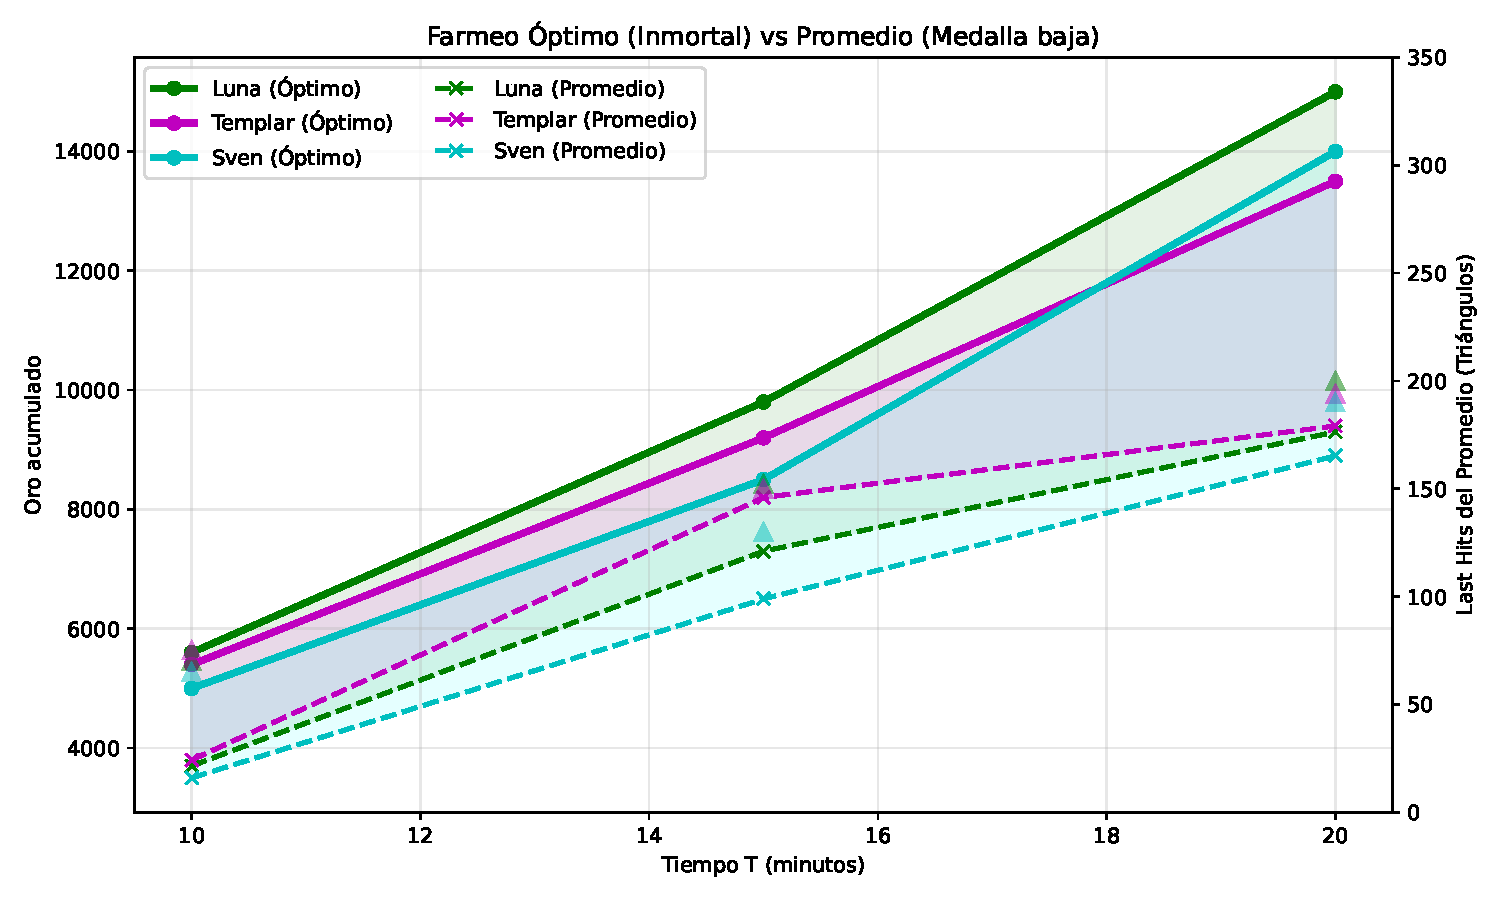
\includegraphics[width=0.85\textwidth]{../figuras/fopt_vs_freal.pdf}
    \caption{Comparación del oro acumulado: rendimiento de un jugador Inmortal (líneas sólidas) frente a un jugador promedio (líneas punteadas).}
    \label{fig:fopt_vs_freal}
\end{figure}

El área sombreada bajo las curvas representa el \textbf{oro perdido} por el jugador promedio. Esta brecha demuestra que la diferencia entre un jugador de alto nivel y uno de nivel medio no está en el tiempo de juego, sino en la \textbf{eficiencia de las rotaciones} y el aprovechamiento de habilidades para limpiar oleadas dobles o campamentos apilados.
\subsection{Evolución del error relativo}

La Figura \ref{fig:error_relativo} presenta la evolución del error relativo \(E_r(T)\) para los tres héroes. Se observa que, en todos los casos, el error tiende a incrementarse con el tiempo, aunque a ritmos distintos según el estilo de farmeo de cada héroe.

\begin{figure}[htbp]
    \centering
    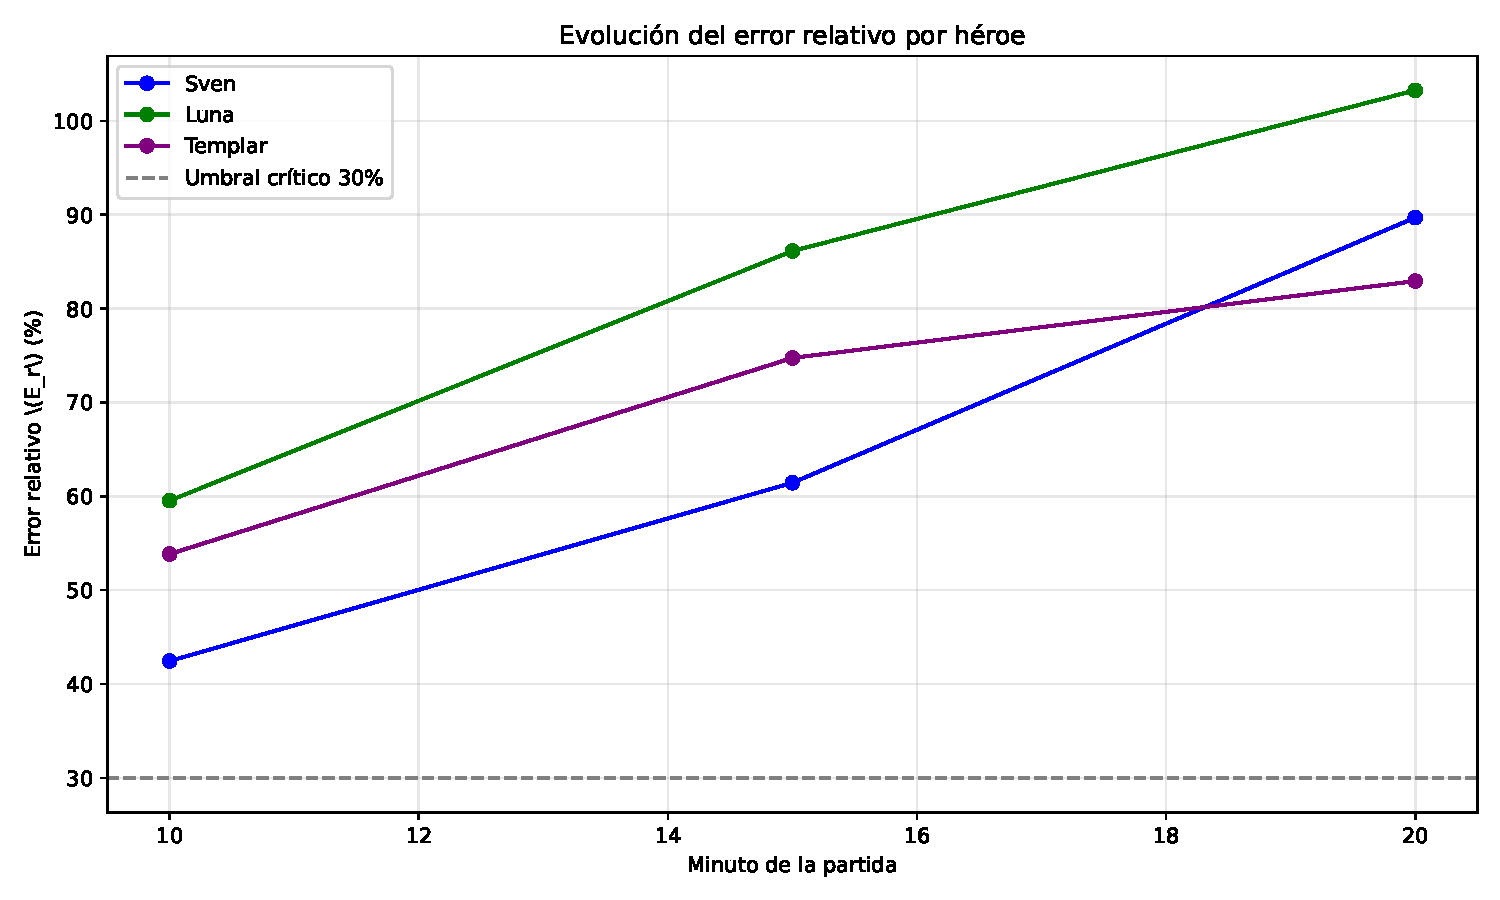
\includegraphics[width=0.85\textwidth]{../figuras/error_relativo.pdf}
    \caption{Evolución del error relativo por héroe a lo largo de la partida.}
    \label{fig:error_relativo}
\end{figure}

\textbf{Luna} presenta el error relativo más bajo en los primeros 10 minutos, lo que es consistente con su estilo de farmeo a distancia y su capacidad de limpiar campamentos sin exponerse demasiado. \textbf{Templar Assassin}, en cambio, muestra un crecimiento más pronunciado del error, posiblemente porque su dependencia del posicionamiento preciso la hace más vulnerable a perder eficiencia cuando la ruta no se ejecuta con exactitud. \textbf{Sven} se mantiene en un punto intermedio, beneficiándose de su daño en área pero limitado por su naturaleza cuerpo a cuerpo.

\subsection{Interpolación del oro acumulado}

La Figura \ref{fig:interpolacion} ilustra el uso de la interpolación de Lagrange para estimar el oro acumulado en minutos no medidos directamente. A partir de tres puntos conocidos (minutos 5, 10 y 15), se construye una curva polinómica que permite estimar el valor en el minuto 12.

\begin{figure}[htbp]
    \centering
    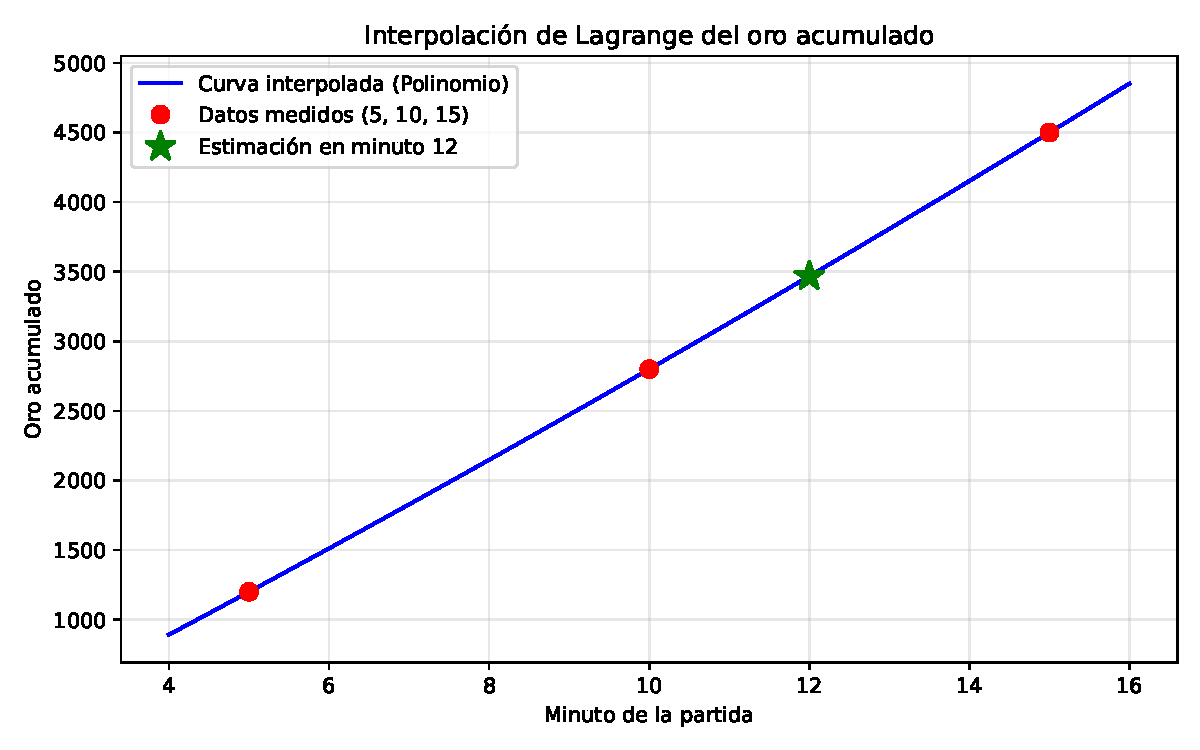
\includegraphics[width=0.75\textwidth]{../figuras/interpolacion.pdf}
    \caption{Interpolación de Lagrange aplicada a los datos de oro acumulado.}
    \label{fig:interpolacion}
\end{figure}

Este procedimiento permite construir una función continua de rendimiento a partir de datos discretos, lo que facilita la comparación con la curva teórica \(F_{opt}(T)\) y la identificación de los momentos en que el farmeo real se desvía del óptimo.

\subsection{Grafo de rutas de farmeo}

La Figura \ref{fig:grafo_rutas} muestra el grafo simplificado de rutas construido para modelar los desplazamientos entre la línea y los campamentos neutrales. Los nodos representan ubicaciones del mapa y las aristas están ponderadas con los tiempos de desplazamiento medidos.

\begin{figure}[htbp]
    \centering
    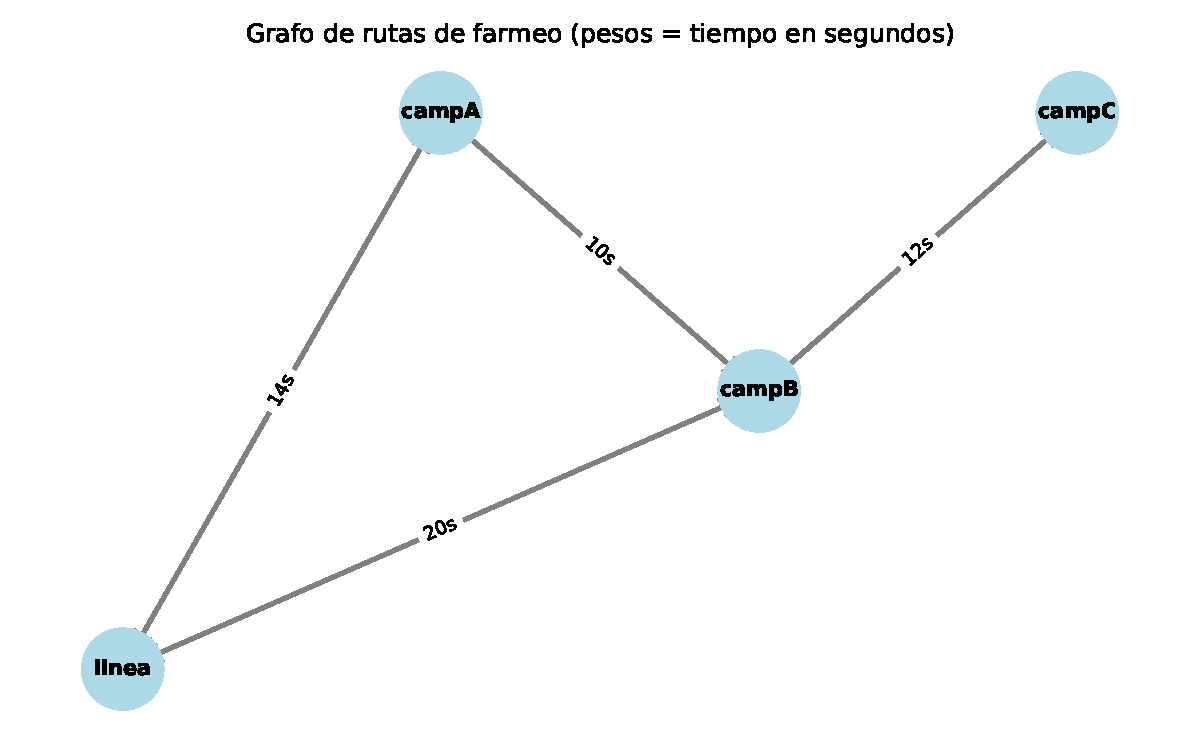
\includegraphics[width=0.75\textwidth]{../figuras/grafo_rutas.pdf}
    \caption{Grafo de rutas de farmeo con pesos temporales.}
    \label{fig:grafo_rutas}
\end{figure}

Sobre este grafo es posible aplicar algoritmos de optimización para determinar la secuencia de nodos que maximiza el oro acumulado, respetando las restricciones temporales impuestas por la aparición de oleadas y campamentos.